% SAT-SA manuscript -- IEEE Access (Applied Research) submission wrapper.
% Built into paper/submission/manuscript.tex by paper/make_submission.py.
% Body text is paper/sections/*.tex, shared with the venue-neutral manuscript.
% Every result number is a \V{claim-id} macro from data/values.tex, generated
% from research/evidence/freeze-v2 by scripts/build_paper_assets.py.
\documentclass{ieeeaccess}
\usepackage{cite}
\usepackage{amsmath,amssymb,amsfonts}
\usepackage{graphicx}
\usepackage{textcomp}
\usepackage{booktabs,adjustbox,url}
% Figure 1 is a pre-rendered PDF (figures-src/): TikZ fails under ieeeaccess.cls.
% Generated from paper/data/paper-data.json; do not edit.
% Freeze: satsa-evidence-freeze-v2
\makeatletter
\newcommand{\V}[1]{\@ifundefined{pv@#1}{\PackageError{paperdata}{Undefined paper value #1}{}}{\@nameuse{pv@#1}}}
\@namedef{pv@CODE-workers}{16}
\@namedef{pv@CODE-dimensions}{7}
\@namedef{pv@CODE-graph-nodes}{5}
\@namedef{pv@CODE-signature}{ML-DSA-65}
\@namedef{pv@CODE-api-routes}{44}
\@namedef{pv@C01-tp}{5}
\@namedef{pv@C01-fp}{7}
\@namedef{pv@C01-fn}{0}
\@namedef{pv@C01-precision}{0.417}
\@namedef{pv@C01-recall}{1.000}
\@namedef{pv@C01-f1}{0.588}
\@namedef{pv@C01-action-ok}{4}
\@namedef{pv@C01-action-total}{5}
\@namedef{pv@C01-catalog-size}{10}
\@namedef{pv@C01-closure-n}{12}
\@namedef{pv@C01-closure-pos}{3}
\@namedef{pv@C01-closure-f1-satsa}{1.00}
\@namedef{pv@C01-closure-f1-fixed}{1.00}
\@namedef{pv@C01-closure-f1-mad}{1.00}
\@namedef{pv@C01-closure-f1-random}{0.33}
\@namedef{pv@C01-closure-recall-zscore}{0.0}
\@namedef{pv@C01-closure-recall-iqr}{0.0}
\@namedef{pv@R01b-expect}{245}
\@namedef{pv@R01b-match}{245}
\@namedef{pv@R01b-na}{3}
\@namedef{pv@R01b-missingness-n}{173}
\@namedef{pv@R01b-missingness-analysed}{140}
\@namedef{pv@R01b-missingness-changed}{43}
\@namedef{pv@R01b-missingness-invalid}{33}
\@namedef{pv@R01b-duplication-n}{34}
\@namedef{pv@R01b-duplication-analysed}{9}
\@namedef{pv@R01b-duplication-changed}{5}
\@namedef{pv@R01b-duplication-invalid}{25}
\@namedef{pv@R01b-malformation-n}{15}
\@namedef{pv@R01b-malformation-analysed}{0}
\@namedef{pv@R01b-malformation-changed}{0}
\@namedef{pv@R01b-malformation-invalid}{15}
\@namedef{pv@R01b-staleness-n}{15}
\@namedef{pv@R01b-staleness-analysed}{15}
\@namedef{pv@R01b-staleness-changed}{0}
\@namedef{pv@R01b-conflict-n}{18}
\@namedef{pv@R01b-conflict-analysed}{13}
\@namedef{pv@R01b-conflict-changed}{4}
\@namedef{pv@R01b-conflict-invalid}{5}
\@namedef{pv@R01b-control-n}{5}
\@namedef{pv@R01b-control-analysed}{5}
\@namedef{pv@R01b-control-changed}{0}
\@namedef{pv@R01b-ind10-rejected}{3}
\@namedef{pv@R01b-ind10-changed}{0}
\@namedef{pv@R01b-ind25-rejected}{11}
\@namedef{pv@R01b-ind25-changed}{4}
\@namedef{pv@R01b-ind50-rejected}{14}
\@namedef{pv@R01b-ind50-changed}{4}
\@namedef{pv@R01b-cas10-rejected}{0}
\@namedef{pv@R01b-cas10-changed}{1}
\@namedef{pv@R01b-cas25-rejected}{0}
\@namedef{pv@R01b-cas25-changed}{11}
\@namedef{pv@R01b-cas50-rejected}{0}
\@namedef{pv@R01b-cas50-changed}{15}
\@namedef{pv@R01b-stale-unchanged}{15}
\@namedef{pv@O01-direct-median}{1.276}
\@namedef{pv@O01-direct-p95}{2.010}
\@namedef{pv@O01-direct-db}{420}
\@namedef{pv@O01-direct-outside}{0.055}
\@namedef{pv@O01-graph-median}{1.433}
\@namedef{pv@O01-graph-p95}{2.206}
\@namedef{pv@O01-graph-db}{458}
\@namedef{pv@O01-graph-outside}{0.115}
\@namedef{pv@O01-unrev-median}{0.976}
\@namedef{pv@O01-unrev-p95}{1.655}
\@namedef{pv@O01-unrev-db}{253}
\@namedef{pv@O01-unrev-outside}{0.029}
\@namedef{pv@O01-checkpoints}{7}
\@namedef{pv@O01-diff-proc}{0.096}
\@namedef{pv@O01-diff-proc-lo}{\ensuremath{-}0.020}
\@namedef{pv@O01-diff-proc-hi}{0.211}
\@namedef{pv@O01-diff-proc-greater}{19}
\@namedef{pv@O01-diff-outside}{0.059}
\@namedef{pv@O01-diff-outside-lo}{0.057}
\@namedef{pv@O01-diff-outside-hi}{0.061}
\@namedef{pv@O01-diff-outside-greater}{30}
\@namedef{pv@O01-diff-db}{38}
\@namedef{pv@O01-diff-db-greater}{30}
\@namedef{pv@O01-diff-review}{0.318}
\@namedef{pv@O01-diff-review-lo}{0.176}
\@namedef{pv@O01-diff-review-hi}{0.569}
\@namedef{pv@O01-diff-review-greater}{26}
\@namedef{pv@O01-diff-proc-rel}{7.5\%}
\@namedef{pv@O01-pairs}{30}
\@namedef{pv@O01-final-median}{0.288}
\@namedef{pv@O01-final-p95}{0.504}
\@namedef{pv@O01-final-share}{23\%}
\@namedef{pv@O01-verify-median}{0.062}
\@namedef{pv@O01-attest-median}{0.853}
\@namedef{pv@O01-sign-calls}{5}
\@namedef{pv@O01-analysis-median}{0.071}
\@namedef{pv@O02-points}{6}
\@namedef{pv@O02-runs}{36}
\@namedef{pv@O02-recovered}{36}
\@namedef{pv@O02-identical}{36}
\@namedef{pv@O02-repeated}{0}
\@namedef{pv@O02-trials}{3}
\@namedef{pv@O02-direct-analysisstagetransient-median}{0.095}
\@namedef{pv@O02-direct-analysisstagetransient-recovered}{3}
\@namedef{pv@O02-direct-analysisstagecrash-median}{0.090}
\@namedef{pv@O02-direct-analysisstagecrash-recovered}{3}
\@namedef{pv@O02-direct-recommendationstransient-median}{0.032}
\@namedef{pv@O02-direct-recommendationstransient-recovered}{3}
\@namedef{pv@O02-direct-workerrestartatreview-median}{1.337}
\@namedef{pv@O02-direct-workerrestartatreview-recovered}{3}
\@namedef{pv@O02-direct-finalizationtransient-median}{1.199}
\@namedef{pv@O02-direct-finalizationtransient-recovered}{3}
\@namedef{pv@O02-direct-finalizationcrash-median}{1.285}
\@namedef{pv@O02-direct-finalizationcrash-recovered}{3}
\@namedef{pv@O02-graph-analysisstagetransient-median}{0.125}
\@namedef{pv@O02-graph-analysisstagetransient-recovered}{3}
\@namedef{pv@O02-graph-analysisstagecrash-median}{0.124}
\@namedef{pv@O02-graph-analysisstagecrash-recovered}{3}
\@namedef{pv@O02-graph-recommendationstransient-median}{0.056}
\@namedef{pv@O02-graph-recommendationstransient-recovered}{3}
\@namedef{pv@O02-graph-workerrestartatreview-median}{1.857}
\@namedef{pv@O02-graph-workerrestartatreview-recovered}{3}
\@namedef{pv@O02-graph-finalizationtransient-median}{0.947}
\@namedef{pv@O02-graph-finalizationtransient-recovered}{3}
\@namedef{pv@O02-graph-finalizationcrash-median}{1.376}
\@namedef{pv@O02-graph-finalizationcrash-recovered}{3}
\@namedef{pv@T01-tested}{14}
\@namedef{pv@T01-expected}{13}
\@namedef{pv@T01-detected}{13}
\@namedef{pv@T01-controls}{1}
\@namedef{pv@P01-cells}{96}
\@namedef{pv@P01-emitted-tight}{35}
\@namedef{pv@P01-emitted-wide}{14}
\@namedef{pv@P01-tight-n2}{0}
\@namedef{pv@P01-tight-n3}{7}
\@namedef{pv@P01-tight-n4}{7}
\@namedef{pv@P01-tight-n5}{7}
\@namedef{pv@P01-tight-n6}{7}
\@namedef{pv@P01-tight-n8}{7}
\@namedef{pv@P01-wide-n2}{0}
\@namedef{pv@P01-wide-n3}{2}
\@namedef{pv@P01-wide-n4}{2}
\@namedef{pv@P01-wide-n5}{4}
\@namedef{pv@P01-wide-n6}{3}
\@namedef{pv@P01-wide-n8}{3}
\@namedef{pv@A01-workers}{16}
\@namedef{pv@A01-full-precision}{0.556}
\@namedef{pv@A01-full-recall}{1.000}
\@namedef{pv@A01-full-f1}{0.714}
\@namedef{pv@A01-fast-closure-precision}{0.429}
\@namedef{pv@A01-fast-closure-recall}{0.600}
\@namedef{pv@A01-negative-space-precision}{0.500}
\@namedef{pv@A01-negative-space-recall}{0.600}
\@namedef{pv@A01-evidence-completeness-precision}{0.500}
\@namedef{pv@A01-evidence-completeness-recall}{0.800}
\@namedef{pv@A01-recurring-without-remediation-precision}{0.714}
\@namedef{pv@A01-recurring-without-remediation-recall}{1.000}
\@namedef{pv@A01-coverage-gap-precision}{0.625}
\@namedef{pv@A01-coverage-gap-recall}{1.000}
\@namedef{pv@A01-pop-full}{0.760}
\@namedef{pv@A01-pop-fast-closure}{0.600}
\@namedef{pv@A01-pop-negative-space}{0.640}
\@namedef{pv@A01-pop-peer-benchmark}{0.720}
\@namedef{pv@A01-pop-anomaly}{0.800}
\@namedef{pv@A01-pop-recurring-without-remediation}{0.800}
\@namedef{pv@A01-pop-coverage-gap}{0.800}
\@namedef{pv@A01-pop-workflow-reconstruction}{0.800}
\@namedef{pv@A01-pop-case-similarity}{0.720}
\@namedef{pv@PR01-satsa-precision10}{1.000}
\@namedef{pv@PR01-satsa-recall20}{0.800}
\@namedef{pv@PR01-satsa-ndcg20}{1.000}
\@namedef{pv@PR01-satsa-recall30}{0.800}
\@namedef{pv@PR01-satsa-ndcg30}{0.869}
\@namedef{pv@PR01-satsa-volume}{7.0}
\@namedef{pv@PR01-random-precision10}{0.245}
\@namedef{pv@PR01-random-recall20}{0.201}
\@namedef{pv@PR01-random-ndcg20}{0.248}
\@namedef{pv@PR01-random-recall30}{0.295}
\@namedef{pv@PR01-random-ndcg30}{0.276}
\@namedef{pv@PR01-random-volume}{17.5}
\@namedef{pv@PR01-volume-precision10}{0.500}
\@namedef{pv@PR01-volume-recall20}{0.200}
\@namedef{pv@PR01-volume-ndcg20}{0.246}
\@namedef{pv@PR01-volume-recall30}{0.400}
\@namedef{pv@PR01-volume-ndcg30}{0.318}
\@namedef{pv@PR01-volume-volume}{18.0}
\@namedef{pv@PR01-closure-precision10}{1.000}
\@namedef{pv@PR01-closure-recall20}{0.600}
\@namedef{pv@PR01-closure-ndcg20}{0.832}
\@namedef{pv@PR01-closure-recall30}{0.800}
\@namedef{pv@PR01-closure-ndcg30}{0.837}
\@namedef{pv@PR01-closure-volume}{11.5}
\@namedef{pv@PR01-vs-random-diff}{0.59}
\@namedef{pv@PR01-vs-random-lo}{0.41}
\@namedef{pv@PR01-vs-random-hi}{0.60}
\@namedef{pv@PR01-vs-random-higher}{20}
\@namedef{pv@PR01-vs-random-equal}{0}
\@namedef{pv@PR01-vs-random-lower}{0}
\@namedef{pv@PR01-vs-volume-diff}{0.40}
\@namedef{pv@PR01-vs-volume-lo}{0.30}
\@namedef{pv@PR01-vs-volume-hi}{0.60}
\@namedef{pv@PR01-vs-volume-higher}{20}
\@namedef{pv@PR01-vs-volume-equal}{0}
\@namedef{pv@PR01-vs-volume-lower}{0}
\@namedef{pv@PR01-vs-closure-diff}{0.00}
\@namedef{pv@PR01-vs-closure-lo}{0.00}
\@namedef{pv@PR01-vs-closure-hi}{0.20}
\@namedef{pv@PR01-vs-closure-higher}{8}
\@namedef{pv@PR01-vs-closure-equal}{11}
\@namedef{pv@PR01-vs-closure-lower}{1}
\@namedef{pv@PR01-vs-closure-ndcg30-higher}{12}
\@namedef{pv@PR01-vs-volume-p10-higher}{18}
\@namedef{pv@PR01-vs-closure-ndcg30-equal}{3}
\@namedef{pv@PR01-vs-volume-p10-equal}{2}
\@namedef{pv@PR01-vs-closure-ndcg30-lower}{5}
\@namedef{pv@PR01-vs-volume-p10-lower}{0}
\@namedef{pv@PR01-vol-fewer-closure}{12}
\@namedef{pv@PR01-vol-more-closure}{6}
\@namedef{pv@X02b-groups}{50}
\@namedef{pv@X02b-incidents}{22,604}
\@namedef{pv@X02b-incidents-total}{24,918}
\@namedef{pv@X02b-events}{47,420}
\@namedef{pv@X02b-reassign}{19,656}
\@namedef{pv@X02b-rows-received}{134,888}
\@namedef{pv@X02b-rows-accepted}{134,888}
\@namedef{pv@X02b-rows-rejected}{0}
\@namedef{pv@X02b-analysis-median}{9}
\@namedef{pv@X02b-relevant}{12}
\@namedef{pv@X02b-rho-risk}{\ensuremath{-}0.11}
\@namedef{pv@X02b-rho-risk-lo}{\ensuremath{-}0.42}
\@namedef{pv@X02b-rho-risk-hi}{0.21}
\@namedef{pv@X02b-rho-slowest}{0.94}
\@namedef{pv@X02b-rho-slowest-lo}{0.86}
\@namedef{pv@X02b-rho-slowest-hi}{0.97}
\@namedef{pv@X02b-rho-volume}{\ensuremath{-}0.15}
\@namedef{pv@X02b-rho-volume-lo}{\ensuremath{-}0.42}
\@namedef{pv@X02b-rho-volume-hi}{0.16}
\@namedef{pv@X02b-rho-reassign}{0.37}
\@namedef{pv@X02b-rho-reassign-lo}{0.08}
\@namedef{pv@X02b-rho-reassign-hi}{0.60}
\@namedef{pv@X02b-p10-satsa}{0.40}
\@namedef{pv@X02b-p10-random}{0.25}
\@namedef{pv@X02b-p10-slowest}{1.00}
\@namedef{pv@X02b-volume-satsa}{50}
\@namedef{pv@X02b-volume-slowest}{24}
\@namedef{pv@X03-saturated}{4}
\@namedef{pv@X03-zero-dims}{3}
\@namedef{pv@X03-rho-fast}{\ensuremath{-}0.70}
\@namedef{pv@X03-rho-fast-lo}{\ensuremath{-}0.82}
\@namedef{pv@X03-rho-fast-hi}{\ensuremath{-}0.52}
\@namedef{pv@X03-rho-resolution}{0.94}
\@namedef{pv@X03-rho-resolution-lo}{0.86}
\@namedef{pv@X03-rho-resolution-hi}{0.97}
\@namedef{pv@X03-rho-nosteps}{\ensuremath{-}0.12}
\@namedef{pv@X03-rho-nosteps-lo}{\ensuremath{-}0.41}
\@namedef{pv@X03-rho-nosteps-hi}{0.18}
\@namedef{pv@X03-rho-execgap}{\ensuremath{-}0.41}
\@namedef{pv@X03-rho-execgap-lo}{\ensuremath{-}0.66}
\@namedef{pv@X03-rho-execgap-hi}{\ensuremath{-}0.11}
\@namedef{pv@X03-risk-distinct}{49}
\@namedef{pv@X03-risk-vs-volume}{0.02}
\@namedef{pv@X03-cases-min}{1.7\%}
\@namedef{pv@X03-cases-max}{78.4\%}
\@namedef{pv@X03-alerts-min}{5.2\%}
\@namedef{pv@X03-alerts-max}{85.9\%}
\@namedef{pv@X03-missed}{7,907}
\@namedef{pv@X03-other-group}{3}
\@namedef{pv@X03-reassigned-miss}{53.8\%}
\@namedef{pv@X03-notreassigned-miss}{21.5\%}
\@namedef{pv@X03-note-rule}{39}
\@namedef{pv@D01-pass}{18}
\@namedef{pv@D01-fail}{0}
\@namedef{pv@D01-notrun}{0}
\@namedef{pv@PR01-replicates}{20}
\@namedef{pv@PR01-entities}{20}
\@namedef{pv@PR01-pathological}{5}
\@namedef{pv@CODE-registry}{32}
\@namedef{pv@CODE-registry-satsa}{23}
\@namedef{pv@CODE-registry-mlops}{9}
\@namedef{pv@RISK-w-execution-gap}{25}
\@namedef{pv@RISK-w-peer-deviation}{20}
\@namedef{pv@RISK-w-detection-gap}{15}
\@namedef{pv@RISK-w-negative-space}{15}
\@namedef{pv@RISK-w-anomaly}{15}
\@namedef{pv@RISK-w-investigation-quality}{5}
\@namedef{pv@RISK-w-escalation-discipline}{5}
\makeatother


% Figures use the full column width in two-column layout.
\newcommand{\figscale}[1]{1}
% Generated tables open a single-column table float; \widetable sets one across
% both columns without editing the generated file.
\makeatletter
\newcommand{\widetable}[1]{\begingroup
  \expandafter\let\expandafter\table\csname table*\endcsname
  \expandafter\let\expandafter\endtable\csname endtable*\endcsname
  \input{#1}\endgroup}
\makeatother

\begin{document}
\history{Date of publication xxxx 00, 0000, date of current version xxxx 00, 0000.}
\doi{10.1109/ACCESS.2024.0429000}

\title{Record-Level Supervisory Analytics for Security Operations Centres:
Controlled Evaluation, Cryptographic Decision Binding, and an External Negative Result}

% AUTHORS: the author block below is copied from the venue-neutral manuscript.
% Full names, affiliations, e-mail, IEEE membership and ORCID must be supplied
% by the authors; nothing here was inferred from repository or Git metadata.
\author{\uppercase{PrathamKapoor}\authorrefmark{1}}
\address[1]{[Affiliation and e-mail to be supplied by the authors]}
\tfootnote{[Funding statement to be supplied by the authors, or ``This work
received no external funding.'']}

\markboth
{PrathamKapoor: Record-Level Supervisory Analytics for Security Operations Centres}
{PrathamKapoor: Record-Level Supervisory Analytics for Security Operations Centres}

\corresp{Corresponding author: PrathamKapoor ([e-mail to be supplied]).}

\begin{abstract}
Supervisors of security operations centres must periodically judge whether monitored
organizations detect, investigate, escalate and close security work properly, yet
common instruments are self-assessed maturity models and manual record review. We
describe SAT-SA, a system that analyses the operational records an organization
submits each period (alerts, cases, investigation steps, escalations, dispositions,
assets) with \V{CODE-workers} deterministic analytical workers, produces findings that
cite those records, ranks entities by risk, requires a human supervisory decision,
and binds the reviewed state with a post-quantum signed, hash-chained receipt. All
results come from frozen, hash-verified experiment bundles. In \V{C01-action-total}
controlled scenarios the system emitted every declared finding family (recall
\V{C01-recall}, precision \V{C01-precision}), but simple fixed-threshold and
median-deviation rules tied its fast-closure detector. Across \V{PR01-replicates}
generated populations its ranking exceeded random and alert-volume ordering, while a
closure-speed heuristic was comparable. Validation matched its declared contract in
all \V{R01b-expect} perturbed conditions, yet stale and contradictory records were
accepted silently. The integrity layer detected all \V{T01-detected} tested
mutations, and all \V{O02-runs} injected workflow interruptions recovered. On a real
public service-desk incident log, which is not security operations data, the
pipeline processed every record, but its risk score was not associated with
service-level misses (Spearman correlation \V{X02b-rho-risk}); a failure analysis
attributes this mainly to construct mismatch. The evidence supports mechanism-level
claims under controlled conditions and feasibility on external data, not
effectiveness in real security operations: no human study or expert labels exist, and
deployment beyond local processes is unverified.

\end{abstract}

\begin{keywords}
Alert prioritization, decision support, human-in-the-loop, negative results,
post-quantum signatures, process conformance, provenance, security operations center,
supervisory analytics, tamper-evident records
\end{keywords}

\titlepgskip=-21pt

\maketitle

\section{Introduction}
\label{sec:intro}

Security operations centres (SOCs) triage large alert volumes under limited analyst
capacity~\cite{vielberth2020soc,tariq2025alertfatigue}, and qualitative studies
document recurring process problems: false-positive-dominated alarms, mismatched
expectations between SOC staff and management, and burnout~\cite{alahmadi2022falsepositives,kokulu2019soc,sundaramurthy2015burnout}.
When an external body supervises many SOCs---for example a national authority
responsible for critical infrastructure---it needs to judge periodically whether
each monitored organization actually investigated, escalated and closed its work
properly. The instruments available for this are mostly maturity self-assessments
such as SOC-CMM~\cite{vanos2016soccmm}, metric catalogues~\cite{forsberg2023metrics},
analyst-performance models~\cite{agyepong2023analyst}, and manual examination of
records. Automated assessment of an incident-management process against a reference
model has been demonstrated for auditors~\cite{palma2024compliance}, and the
performance of an operational SOC has been measured by injecting synthetic
attacks~\cite{rosso2020saibersoc}.

This paper studies a narrower, record-level question: \emph{can a system analyse
the operational records an organization submits each period and produce
evidence-cited supervisory findings and priorities, while leaving the decision
to a human supervisor and making the reviewed state verifiable afterwards---and
how does such a system behave under controlled perturbation and on independent
data?} We describe SAT-SA, an implementation of this workflow built for the Smart
India Hackathon problem SIH26157, and report what a frozen evaluation of it shows
and does not show.

The paper's emphasis is the evidence rather than the architecture. Every number
comes from a hash-verified experiment bundle; negative findings are reported with
the same prominence as positive ones. Three of them bound the conclusions:
simple baselines match parts of SAT-SA on controlled data; stale and contradictory
evidence is accepted silently; and on a real external IT incident log SAT-SA's risk
was not associated with the outcome available there, for reasons we diagnose.

\paragraph{Contributions.}
We separate contribution types explicitly (Section~\ref{sec:discussion} returns to
their strength):
\begin{itemize}
\item \emph{Application framing (candidate, low confidence):} SOC supervision posed as
  record-level analytics for an external supervisor, producing findings that cite
  the submitted records they depend on. The underlying techniques---conformance-style
  absence checks, robust deviation rules, peer comparison---are established, and
  record-based compliance assessment of incident management for auditors
  exists~\cite{palma2024compliance}; the framing is a combination of known parts.
\item \emph{Empirical findings:} controlled evaluations of detection against declared
  labels and simple baselines, one-component ablation, imperfect-evidence robustness,
  peer-cohort sensitivity, orchestration overhead and recovery, and an external
  negative result with a failure analysis.
\item \emph{Engineering:} a tenant-aware submission, analysis and review workflow with
  a durable queue and a LangGraph review interrupt.
\item \emph{Security capability (integration):} supervisory decisions bound to the
  analysed state with standard primitives (SHA3-256, ML-DSA-65) and a hash-chained
  ledger, evaluated with a mutation matrix.
\item \emph{Reproducibility infrastructure:} write-once experiment bundles, an evidence
  freeze with verification, and a paper data layer that generates every reported
  number.
\end{itemize}

We make no claim of novelty, superiority, real-world SOC effectiveness or
large-scale operational use; Section~\ref{sec:limitations} lists what the evidence
does not support.

\section{Research Gap and Related Work}
\label{sec:related}

\paragraph{Search method.}
We positioned SAT-SA with a structured search rather than a systematic review. On
27 September 2026 we ran 20 queries covering SOC assessment and metrics, alert
prioritization and alert fatigue, security process mining and conformance checking,
peer-group analytics, supervisory technology, and tamper-evident and post-quantum
audit records. Each query was run against OpenAlex (title and abstract) and Crossref,
and the 25 top-ranked records per query and source were retrieved. This gave 656
unique records after deduplication. One screener read every title and, for 106
records, the abstract; 51 records were included and joined with the 26 sources of an
earlier focused review. arXiv throttled the automated queries and was not searched,
and records beyond rank 25 were not screened. The absence of a work in this search
is therefore not evidence that it does not exist. Queries, counts, screening
decisions with reasons, and a comparison matrix are in the supplementary material.

\paragraph{SOC assessment and performance measurement.}
SOC-CMM scores capability maturity across business, people, process, technology and
services domains through a self-assessment tool~\cite{vanos2016soccmm}, and
CTI-SOC2M2 uses the degree of threat-intelligence integration as a proxy for SOC
service maturity~\cite{schlette2021ctisoc2m2}. Agyepong et al.\ review SOC analyst
challenges and metrics~\cite{agyepong2019review} and weight analyst-performance
indicators using a Delphi panel and the analytic hierarchy
process~\cite{agyepong2023analyst}; Forsberg and Frantti derive technical SOC
metrics through design science~\cite{forsberg2023metrics}. A case study in one
academic SOC found that analysts who scored well on key performance indicators did
not necessarily further the SOC's goals~\cite{morin2025mismatched}, which cautions
against reading operational metrics as quality. SAIBERSOC evaluates the performance
of operational SOCs empirically by injecting synthetic attacks and measuring outputs
such as detection accuracy and time to investigation, with 124 students acting as
analysts~\cite{rosso2020saibersoc}. Surveys and qualitative studies characterize SOC
building blocks, challenges and human
factors~\cite{vielberth2020soc,kokulu2019soc,sundaramurthy2015burnout,sundaramurthy2016contradictions}.
These instruments measure maturity, define metrics, explain practice or test a SOC
by injection. None of them computes findings from records that a monitored SOC
submits to an external supervisor.

\paragraph{Record-based assessment of incident handling.}
The closest prior work is the compliance assessment system of Palma et
al.~\cite{palma2024compliance}. It aligns an organization's incident-management
event log with a reference process derived from frameworks such as ITIL and ISO
27035, classifies deviations with a taxonomy, prioritizes them with a cost model,
and supports an auditor. It was validated on a benchmark and demonstrated on a public
real incident-management log. A companion benchmark compares such process-based
assessment models quantitatively~\cite{palma2024benchimp}. Automated, record-based
assessment of how incidents were handled, aimed at an auditor, therefore already
exists. Earlier work applied process mining to IT incident management against
ITIL~\cite{ferreira2008itil} and to security audit trails~\cite{vanderaalst2005security}.
Recent work represents incident-response activities and responder communications
from tool logs as a knowledge graph for process analysis~\cite{galadima2026irgraph},
and DomainPrio analyses the population of a SOC's investigations rather than single
alerts~\cite{chiba2022domainprio}. SAT-SA differs from Palma et al.\ in mechanism
and scope rather than in kind. It uses rule-encoded checks over SOC evidence
categories (alerts, cases, investigation steps, escalations, dispositions, assets)
instead of alignment with a process model. It compares an entity with a declared peer
cohort, ranks monitored organizations by a fused risk, and binds the supervisor's
decision to the analysed state cryptographically. We did not compare SAT-SA with
that system experimentally.

\paragraph{Alert prioritization and alert fatigue.}
A large literature ranks alerts or incidents for SOC analysts. Jalalvand et
al.\ review 89 prioritization papers through a human--AI teaming
lens~\cite{jalalvand2024prioritisation}, and Tariq et al.\ survey alert-fatigue
mitigations~\cite{tariq2025alertfatigue}. Systems include resource-aware
optimization of which alerts to investigate~\cite{shah2019alertselection},
provenance-based triage (NoDoze~\cite{hassan2019nodoze}), guided response trained on
customer triage labels~\cite{freitas2024guide}, large-scale incident
ranking~\cite{freitas2026aip} and learning to defer to analysts~\cite{jalalvand2025l2d}.
SAT-SA differs in unit and user: it ranks \emph{monitored organizations} for a
\emph{supervisor} from rule-based findings about how work was handled, not individual
alerts for an analyst. It is not a competitor to these systems and is not compared
with them.

\paragraph{Process analytics and absence detection.}
Process mining discovers and checks processes from event
logs~\cite{vanderaalst2016pm}. Conformance checking relates recorded behaviour to a
model and exposes skipped or out-of-order
activities~\cite{rozinat2008conformance,carmona2018conformance}. SAT-SA's
execution-gap and ``negative-space'' workers are rule-encoded conformance checks (for
example, an acknowledged alert whose case has no investigation step). We treat them
as an adaptation of this prior art, not a new technique.

\paragraph{Peer comparison and robust deviation.}
Peer group analysis flags entities that diverge from similar entities over
time~\cite{weston2008pga}, in the broader statistical fraud-detection
tradition~\cite{bolton2002fraud}. SAT-SA's peer worker compares an entity with a
declared cohort using the median and the median absolute deviation
(MAD)~\cite{leys2013mad}, with a minimum cohort size and tenant isolation.

\paragraph{Supervisory technology and human oversight.}
Financial supervisors increasingly use technology to analyse regulated entities'
data (``suptech'')~\cite{broeders2018suptech}, and human supervisory judgement
remains indispensable there, as in SAT-SA's design. Automation bias in human use of
decision support~\cite{parasuraman2010automation} has been reviewed specifically for
SOCs~\cite{tilbury2024automationbias}; it motivates keeping the decision with the
supervisor, and it was not studied here.

\paragraph{Integrity and provenance of records.}
Forward-secure and tamper-evident logs detect alteration of recorded
history~\cite{schneier1999logs,crosby2009logging}. Practical systems protect
operating-system audit logs with trusted execution~\cite{paccagnella2020custos} or
combine ratcheting with keystream storage~\cite{guardiola2022sealfs}, and recent work
applies post-quantum primitives to tamper-evident forensic logging in the
cloud~\cite{fugkeaw2026pqabl}. W3C PROV provides a provenance
vocabulary~\cite{w3c2013provdm}. SAT-SA does not propose a logging scheme or new
cryptography. It composes standard primitives, SHA3-256~\cite{nist2015fips202} and
ML-DSA-65~\cite{nist2024fips204}, to bind one canonical supervisory record to the
authorized decision.

\paragraph{Gap, stated conservatively.}
Record-based assessment of incident handling~\cite{palma2024compliance}, supervisory
analysis of submitted data~\cite{broeders2018suptech}, peer comparison and
tamper-evident records each exist. In the structured search we did not find a work
that combines them in the way SAT-SA does: supervisor-side analysis of SOC evidence
submissions across monitored organizations, with record-cited findings, peer-cohort
comparison, entity risk ranking and a cryptographically bound human decision. This
is a combination of established parts, identified by a search with the limits
stated above. We therefore offer the framing only as a low-confidence candidate
contribution and make no novelty claim.

\section{System Architecture}
\label{sec:architecture}

\begin{figure}[t]
\centering
% TikZ source: figures-src/fig-architecture.tex (values from data/values.tex).
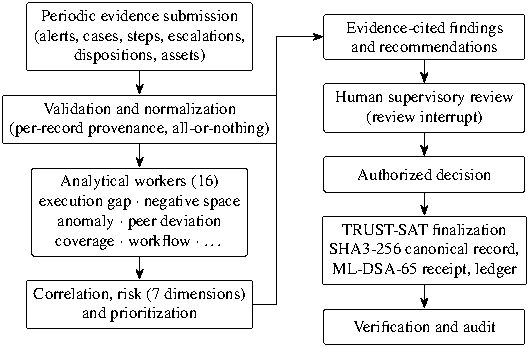
\includegraphics[width=\linewidth,height=62mm,keepaspectratio]{figures-static/fig-architecture.pdf}
\caption{SAT-SA supervisory workflow as implemented. Analytics are deterministic;
orchestration (direct worker or LangGraph) sequences the stages and pauses for the
human decision.}
\label{fig:architecture}
\end{figure}

Figure~\ref{fig:architecture} shows the workflow; Table~\ref{tab:system} lists the
facts the experiments rely on, generated from the source code.

\paragraph{Submission and validation.}
An analyst of the monitored organization creates a versioned submission for an
assessment period and uploads one file per evidence category through an HTTP API
(\V{CODE-api-routes} routes). Validation parses each record, resolves references
(an investigation step must reference an existing case), enforces chronology
(closure not before acknowledgement) and stores per-record source provenance
(artifact digest, record locator). Hosted validation is all-or-nothing: any
rejected record invalidates the version. Artifacts are stored in local storage or
an S3-compatible object store; metadata in SQLite or PostgreSQL.

\paragraph{Analysis.}
A separate worker process claims queued runs with a lease and executes
\V{CODE-workers} deterministic analytical workers over the version's canonical
records. Each emits findings with a rationale, statistic, threshold, confidence
vector and references to the source records it depends on; a signal finding
without evidence references is invalid and is withheld. No worker uses a language
model; LangGraph is used only for orchestration. The repository's capability
registry lists \V{CODE-registry} components (\V{CODE-registry-satsa} supervisory
components and \V{CODE-registry-mlops} retained machine-learning-operations agents);
the experiments exercise the \V{CODE-workers} default analytical workers and the
workflow around them, not every registered component.

\paragraph{Risk and prioritization.}
Findings are grouped into \V{CODE-dimensions} weighted dimensions (execution gap,
peer deviation, detection gap, negative space, anomaly, investigation quality,
escalation discipline). Each dimension's score saturates in the summed
confidence of its findings, and the total (capped at 100) orders entities for
supervisory attention. Findings receive recommendations.

\paragraph{Human review and orchestration.}
Runs can require review. In \emph{direct} mode the worker pauses the run after
analysis and recommendations; in \emph{graph} mode a LangGraph graph with
\V{CODE-graph-nodes} nodes (readiness, analysis, recommendations, human review,
trust boundary) checkpoints its state and interrupts at the review node~\cite{langgraph2026docs}.
Only a supervisor (or organization administrator) can record the decision; the worker then
resumes.

\paragraph{TRUST-SAT finalization and verification.}
After the decision, the system builds a canonical supervisory document
(run, decision, finding, observation, risk and recommendation digests, submission
snapshot and source provenance), hashes it with SHA3-256, signs the digest with
\V{CODE-signature}, stores a receipt, and appends the event to a hash-chained
ledger. Verification rebuilds the document from live records and checks digest,
decision binding, signature and ledger chain (Section~\ref{sec:integrity}).

\paragraph{Deployment.}
The repository contains a container image, a compose topology (PostgreSQL,
SeaweedFS object storage, migration and key-initialization jobs, API, worker) and a
continuous-integration (CI) job that would run it. All measurements in this paper were taken with SQLite and
local storage on one machine; the containerized topology, live PostgreSQL and live
S3 storage were not executed (Table~\ref{tab:deployment}).

\widetable{tables/tab-system}

\section{Analytical Methodology}
\label{sec:analytics}

The workers fall into rule families that the experiments exercise directly.

\paragraph{Execution gaps.} Rules over individual records: an alert closed faster
than a severity-specific limit (e.g.\ critical within ten minutes, above a floor),
an acknowledged medium-or-higher alert whose case has fewer than two investigation
steps, a critical alert without escalation, repeated shallow investigation patterns,
recurring alerts without remediation, and very high closure rates with little
investigation. Most fire when at least one qualifying record exists
(\emph{existence rules}).

\paragraph{Negative space.} Absence of expected work: cases without investigation
steps, missing escalations or dispositions, and critical assets without alerts.
These are rule-encoded conformance checks~\cite{carmona2018conformance}.

\paragraph{Anomaly and peer deviation.} Within-entity outliers are values more than
three MADs from the entity's median~\cite{leys2013mad}; peer deviation compares an
entity's metric with the median and MAD of a declared cohort of at least three
peers and flags deviations of two MADs or more.

\paragraph{Coverage and completeness.} Assets without monitoring and missing
evidence categories.

\paragraph{Fusion.} Findings from different rule families that name the same
subject are reported as corroborating clusters, which do not change the score;
dimension scores saturate in summed confidence, with weights
\V{RISK-w-execution-gap} (execution gap), \V{RISK-w-peer-deviation} (peer deviation),
\V{RISK-w-detection-gap} (detection gap), \V{RISK-w-negative-space} (negative space),
\V{RISK-w-anomaly} (anomaly), \V{RISK-w-investigation-quality} (investigation quality)
and \V{RISK-w-escalation-discipline} (escalation discipline); the entity ranking
sorts by the total.
A property that matters later: the fusion sums finding confidences and does not
use how \emph{prevalent} a problem is within the submission.

\section{Experimental Design}
\label{sec:design}

\paragraph{Research questions.}
RQ1: does SAT-SA emit the finding families declared for controlled scenarios?
RQ2: how does it compare with simple baselines, and what does each worker
contribute? RQ4: how does it behave on imperfect evidence? RQ5: does verification
detect tampering with the finalized record? RQ6: how sensitive is the peer worker
to cohort size and dispersion? RQ7: what do durable orchestration and review cost,
and do interrupted runs recover? EXT: does the pipeline run on independent real
data, and is its risk associated with an outcome available there? (RQ3, analyst
utility, requires a human study that was not run.) Table~\ref{tab:experiments}
maps questions to experiments.

\widetable{tables/tab-experiments}

\paragraph{Data.}
\emph{Controlled catalog:} \V{C01-action-total} executable scenarios authored
with declared finding families and recommended supervisory actions
(\V{C01-catalog-size} catalog entries in total). Labels are construction labels:
they encode what each scenario was built to contain, so agreement shows the
mechanism responds to its designed inputs, not that it detects real misconduct.
\emph{Generated populations} (PR01): \V{PR01-replicates} populations of
\V{PR01-entities} entities each, \V{PR01-pathological} of them declared
pathological, seeded independently. \emph{Engineered peer cohorts} (P01):
\V{P01-cells} cells crossing cohort size, dispersion and deviation.
\emph{External:} the UCI incident management process event log~\cite{amaral2018uci498}
(dataset 498), a real IT service-desk log of one organization, mapped to SAT-SA
categories by an adapter and analysed per assignment group
(\V{X02b-groups} groups with enough incidents). It is IT incident data, not SOC
data. Two security datasets were assessed and not used: GUIDE~\cite{freitas2024guide}
has real triage-graded SOC incidents but no acknowledgement, closure,
investigation-step or escalation records (and its download requires an
authenticated account), and CIC-IDS2017~\cite{sharafaldin2018cicids} contains
network flows rather than SOC workflow records.

\paragraph{Baselines.}
For closure-time detection: fixed threshold, MAD rule, z-score and
interquartile-range (IQR) rules, and random. For prioritization: random order
(\V{PR01-replicates} populations with repeated random trials), critical-and-high alert volume and a
closure-speed heuristic (fastest median closure time first). Externally: random, volume,
reassignment rate and slowest median resolution---the last is close to the
outcome's own construct and is included as an upper reference, not a competitor.

\paragraph{Metrics.}
Precision, recall and F1 against construction labels; precision, recall and
normalized discounted cumulative gain (NDCG)~\cite{jarvelin2002ndcg} within the top $k\in\{10,20,30\}$\% of entities
(written P@$k$, R@$k$, NDCG@$k$);
review volume needed to find all pathological entities; conformance with the
validation contract and change of emitted finding families relative to a paired control;
wall-clock seconds, database statements and share of time outside the analytics;
Spearman $\rho$ against the share of incidents that missed their service-level
agreement (SLA-miss rate).

\paragraph{Statistics policy.}
We report medians; 95th percentiles only when $n\ge20$; seeded percentile
bootstrap intervals~\cite{efron1993bootstrap} only when $n\ge10$ independent
units; paired differences with counts of units where one arm was higher, equal or
lower; and no $p$-values or multiple-comparison claims. The independent unit is
stated for each experiment (Table~\ref{tab:experiments}); repeated trials within
one population or one workflow are not independent. Analyses are descriptive.

\paragraph{Evidence discipline.}
Each experiment writes a write-once bundle (manifest with code commit and a
dirty-tree flag, configuration, raw results, processed metrics, summary) with
SHA-256 hashes. The canonical bundles are frozen in
\texttt{research/evidence/freeze-v2}; superseded bundles (for example X02,
replaced by X02b after an ingestion-bookkeeping correction that left every
analytical output identical) are kept but not cited for results.
Every number in this paper is rendered from these bundles by the paper data layer
(Section~\ref{sec:repro}).

\section{Results}
\label{sec:results}

\subsection{Controlled detection and closure-time baselines (RQ1, RQ2)}

Over the \V{C01-action-total} controlled scenarios analysed in one shared database,
SAT-SA emitted every declared finding family (true positives \V{C01-tp}, false negatives \V{C01-fn}) and
\V{C01-fp} undeclared families, giving micro precision \V{C01-precision}, recall
\V{C01-recall} and F1 \V{C01-f1}. Its recommended supervisory action matched the
declared action in \V{C01-action-ok} of \V{C01-action-total} scenarios. Precision
depends on the database layout: analysed one scenario per database (A01), the full
worker set had precision \V{A01-full-precision}, because cross-entity workers in the
shared database see other scenarios' records. Because labels are construction
labels, these figures show the mechanism responds to its designed inputs; they
are not accuracy on real SOC data.

On \V{C01-closure-n} construction-labelled critical closures
(\V{C01-closure-pos} fast), SAT-SA's fast-closure detector, a fixed threshold and a
MAD rule each reached F1 \V{C01-closure-f1-satsa}; z-score and IQR rules found none
(recall \V{C01-closure-recall-zscore}) and seeded random reached
\V{C01-closure-f1-random} (Table~\ref{tab:baselines-closure}). \textbf{The detector
ties simple baselines}; it offers no detection advantage on this corpus.

% Generated by scripts/build_paper_assets.py from satsa-evidence-freeze-v2; do not edit.
% Sources: C01=controlled-final-seed-17 (manifest 0ad518882d319dd9)
\begin{table}[t]
\centering\small
\caption{Closure-time detectors on 12 construction-labelled records (C01).}
\label{tab:baselines-closure}
\begin{adjustbox}{max width=\linewidth}
\begin{tabular}{lrrrrrr}
\toprule
Detector & TP & FP & FN & Precision & Recall & F1 \\
\midrule
SAT-SA fast-closure & 3 & 0 & 0 & 1.00 & 1.00 & 1.00 \\
Fixed threshold & 3 & 0 & 0 & 1.00 & 1.00 & 1.00 \\
MAD & 3 & 0 & 0 & 1.00 & 1.00 & 1.00 \\
z-score & 0 & 0 & 3 & -- & 0.00 & -- \\
IQR & 0 & 0 & 3 & -- & 0.00 & -- \\
Seeded random & 1 & 2 & 2 & 0.33 & 0.33 & 0.33 \\
\bottomrule
\end{tabular}
\end{adjustbox}
\par\smallskip\footnotesize Undefined ratios shown as --. SAT-SA ties the fixed-threshold and MAD baselines.
\end{table}


\subsection{Prioritization against simple baselines (RQ2)}

Across \V{PR01-replicates} generated populations, SAT-SA placed a median
\V{PR01-satsa-recall20} of the pathological entities in its top 20\% and needed a
median of \V{PR01-satsa-volume} reviews to find all of them
(Table~\ref{tab:baselines-prioritization}, Figure~\ref{fig:prioritization}).
Versus random order its recall@20\% was higher in \V{PR01-vs-random-higher}
populations and lower in \V{PR01-vs-random-lower} (median paired difference
\V{PR01-vs-random-diff}, 95\% bootstrap \V{PR01-vs-random-lo} to
\V{PR01-vs-random-hi}); versus alert volume, higher in \V{PR01-vs-volume-higher}
and lower in \V{PR01-vs-volume-lower} (difference \V{PR01-vs-volume-diff},
\V{PR01-vs-volume-lo} to \V{PR01-vs-volume-hi}).
\textbf{Against the closure-speed heuristic the comparison is mixed:} recall@20\%
was higher in \V{PR01-vs-closure-higher}, equal in \V{PR01-vs-closure-equal} and
lower in \V{PR01-vs-closure-lower} populations (median difference
\V{PR01-vs-closure-diff}, interval \V{PR01-vs-closure-lo} to
\V{PR01-vs-closure-hi}); NDCG@30\% was higher in
\V{PR01-vs-closure-ndcg30-higher}, equal in \V{PR01-vs-closure-ndcg30-equal} and
lower in \V{PR01-vs-closure-ndcg30-lower}; SAT-SA needed fewer reviews in
\V{PR01-vol-fewer-closure} populations and more in \V{PR01-vol-more-closure}.
A single closure-speed rule captures much of what separates these generator
profiles. The populations come from SAT-SA's own generator, whose pathological
profile injects behaviours its detectors target, so the comparison favours SAT-SA
by construction; intervals are descriptive and uncorrected.

\widetable{tables/tab-baselines-prioritization}

\begin{figure}[t]
\centering
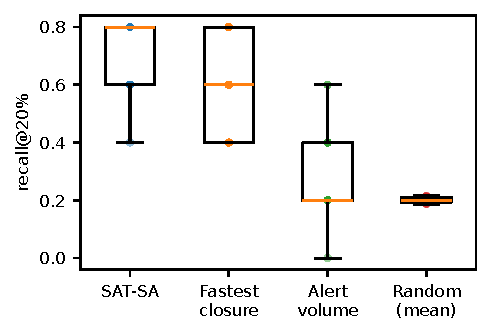
\includegraphics[width=\figscale{0.7}\linewidth]{figures/fig-prioritization.pdf}
\caption{Recall@20\% of generator-labelled pathological entities across generated
populations (PR01).}
\label{fig:prioritization}
\end{figure}

\subsection{Component ablation (RQ2)}

Removing one of the \V{A01-workers} workers at a time (Table~\ref{tab:ablation},
Figure~\ref{fig:ablation}), fast-closure and negative-space carried recall on the
catalog (recall \V{A01-fast-closure-recall} and \V{A01-negative-space-recall}
without them); removing evidence-completeness gave \V{A01-evidence-completeness-recall}.
Removing recurring-without-remediation or coverage-gap \emph{raised} precision
(\V{A01-recurring-without-remediation-precision}, \V{A01-coverage-gap-precision})
because those workers emitted only undeclared families here. On generated
populations (five seeds, exploratory), mean recall@20\% was
\V{A01-pop-full} with all workers, \V{A01-pop-fast-closure} without fast-closure
and \V{A01-pop-negative-space} without negative-space, while removing anomaly,
recurring-without-remediation, coverage-gap or workflow-reconstruction raised it to
\V{A01-pop-anomaly}: these workers add ranking noise on these populations. Several
workers had no measurable effect on these fixtures, which says only that the
fixtures do not exercise them.

% Generated by scripts/build_paper_assets.py from satsa-evidence-freeze-v2; do not edit.
% Sources: A01=EXP-A01-component-ablation (manifest 03632678da62b279)
\begin{table}[t]
\centering\small
\caption{One-worker ablation (A01): scenario micro metrics (5 scenarios) and mean population recall@20\% (5 seeds, exploratory). Workers with no change on either view are omitted.}
\label{tab:ablation}
\begin{adjustbox}{max width=\linewidth}
\begin{tabular}{lrrrr}
\toprule
Worker removed & Precision & Recall & F1 & Pop. R@20\% \\
\midrule
(full set) & 0.556 & 1.000 & 0.714 & 0.76 \\
-- fast-closure & 0.429 & 0.600 & 0.500 & 0.60 \\
-- recurring-without-remediation & 0.714 & 1.000 & 0.833 & 0.80 \\
-- negative-space & 0.500 & 0.600 & 0.545 & 0.64 \\
-- anomaly & 0.556 & 1.000 & 0.714 & 0.80 \\
-- peer-benchmark & 0.556 & 1.000 & 0.714 & 0.72 \\
-- coverage-gap & 0.625 & 1.000 & 0.769 & 0.80 \\
-- case-similarity & 0.556 & 1.000 & 0.714 & 0.72 \\
-- evidence-completeness & 0.500 & 0.800 & 0.615 & 0.76 \\
-- workflow-reconstruction & 0.556 & 1.000 & 0.714 & 0.80 \\
\bottomrule
\end{tabular}
\end{adjustbox}
\end{table}


\begin{figure}[t]
\centering
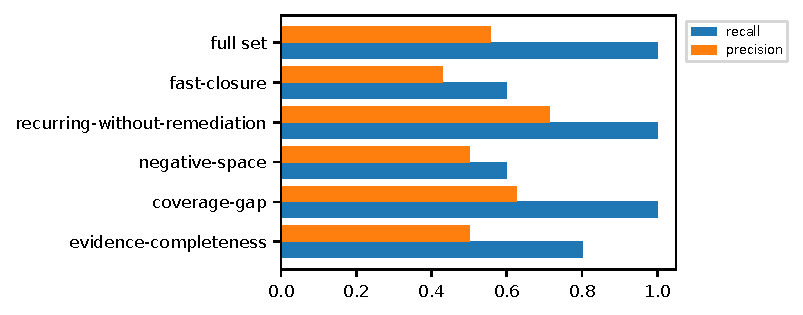
\includegraphics[width=\figscale{0.75}\linewidth]{figures/fig-ablation.pdf}
\caption{Catalog micro precision and recall with one worker removed; unchanged
removals omitted (A01).}
\label{fig:ablation}
\end{figure}

\subsection{Imperfect evidence (RQ4)}

Each of the perturbed conditions declared its family, affected records and
expected validation outcome before it ran, with one fresh tenant database per
condition. Hosted validation matched the declared contract in \V{R01b-match} of
\V{R01b-expect} conditions with an expectation; \V{R01b-na} were not applicable to
their fixture (Table~\ref{tab:robustness}). Exact and conflicting duplicates with
native identifiers, malformed timestamps, chronology violations and missing
columns were rejected (\V{R01b-malformation-invalid} malformation and
\V{R01b-duplication-invalid} duplication conditions).

Two behaviours matter for interpretation (Figure~\ref{fig:robustness}). First,
validation is all-or-nothing: independent record omission left dangling
references and rejected the whole submission in \V{R01b-ind10-rejected},
\V{R01b-ind25-rejected} and \V{R01b-ind50-rejected} of the seeded replicates at
10, 25 and 50\% omission, whereas referentially consistent omission was never
rejected and changed the emitted finding families in \V{R01b-cas10-changed},
\V{R01b-cas25-changed} and \V{R01b-cas50-changed} replicates. Second,
\textbf{stale and contradictory evidence is accepted silently}: all
\V{R01b-staleness-n} conditions with records outside the assessment period were
accepted with no warning and no change to findings or risk
(\V{R01b-stale-unchanged} unchanged), and contradictory dispositions or a closed
case with an open alert produced no finding. SAT-SA implements no period,
recency or cross-record consistency validation.

\widetable{tables/tab-robustness}

\begin{figure}[t]
\centering
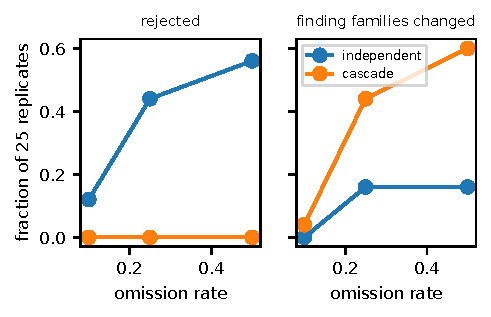
\includegraphics[width=\figscale{0.7}\linewidth]{figures/fig-robustness.pdf}
\caption{Record omission: independent omission is often rejected by all-or-nothing
validation; referentially consistent omission is accepted and changes findings more
often as the rate grows (R01b).}
\label{fig:robustness}
\end{figure}

\subsection{Peer-cohort sensitivity (RQ6)}

Over \V{P01-cells} engineered cells (Table~\ref{tab:peer},
Figure~\ref{fig:peer}), cohorts of two peers never produced a peer finding
(the rule requires three). With a tight cohort spread, \V{P01-tight-n3} of the
eight subject values were flagged from three peers upward---every value except the
one at the cohort median. With a wide spread only extreme slow subjects were
flagged at small cohorts (\V{P01-wide-n3} at three peers), and fast subjects were
flagged only from five peers upward as the MAD narrowed
(\V{P01-wide-n5} at five peers). The rule is therefore sensitive to cohort
dispersion and size, and small or heterogeneous cohorts will miss deviations.

% Generated by scripts/build_paper_assets.py from satsa-evidence-freeze-v2; do not edit.
% Sources: P01=EXP-P01-peer-sweep (manifest 7aa85508062b2b28)
\begin{table}[t]
\centering\small
\caption{Subjects flagged by the peer rule out of 8 subject values per cohort (P01).}
\label{tab:peer}
\begin{adjustbox}{max width=\linewidth}
\begin{tabular}{lrrrrrr}
\toprule
Spread & 2 peers & 3 & 4 & 5 & 6 & 8 \\
\midrule
tight & \V{P01-tight-n2} & \V{P01-tight-n3} & \V{P01-tight-n4} & \V{P01-tight-n5} & \V{P01-tight-n6} & \V{P01-tight-n8} \\
wide & \V{P01-wide-n2} & \V{P01-wide-n3} & \V{P01-wide-n4} & \V{P01-wide-n5} & \V{P01-wide-n6} & \V{P01-wide-n8} \\
\bottomrule
\end{tabular}
\end{adjustbox}
\end{table}


\begin{figure}[t]
\centering
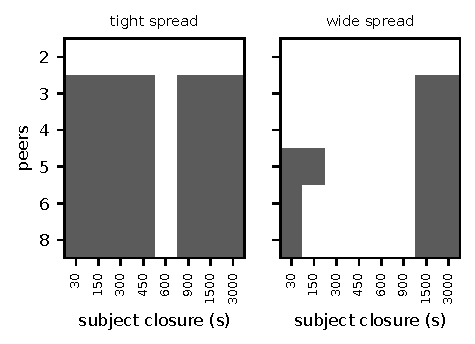
\includegraphics[width=\figscale{0.85}\linewidth]{figures/fig-peer.pdf}
\caption{Peer findings by cohort size, spread and subject closure value; dark cells
emitted a finding (P01).}
\label{fig:peer}
\end{figure}

\subsection{Orchestration cost and recovery (RQ7)}

On one machine with SQLite, \V{O01-pairs} paired trials per mode
(Table~\ref{tab:orchestration}, Figure~\ref{fig:orchestration}) gave median
processing times, excluding the human decision, of \V{O01-direct-median}\,s
(direct), \V{O01-graph-median}\,s (LangGraph) and \V{O01-unrev-median}\,s
(unreviewed benchmark mode). LangGraph minus direct was a median
\V{O01-diff-proc}\,s per workflow (\V{O01-diff-proc-rel} of the direct median; 95\%
bootstrap \V{O01-diff-proc-lo} to \V{O01-diff-proc-hi}\,s, graph slower in
\V{O01-diff-proc-greater} of \V{O01-pairs} pairs), with \V{O01-diff-db} more
database statements and \V{O01-checkpoints} checkpoints per run. Findings and risk
were identical across modes in every trial. Human review with TRUST-SAT
finalization added a median \V{O01-diff-review}\,s over unreviewed processing
(\V{O01-diff-review-lo} to \V{O01-diff-review-hi}\,s); finalization took a median
\V{O01-final-median}\,s (\V{O01-final-share} of reviewed processing), receipt
verification \V{O01-verify-median}\,s, and run and finding attestation
(\V{O01-attest-median}\,s) was the largest single cost. These are repeated
measurements on one machine; the intervals describe that variability only.

\widetable{tables/tab-orchestration}

\begin{figure}[t]
\centering
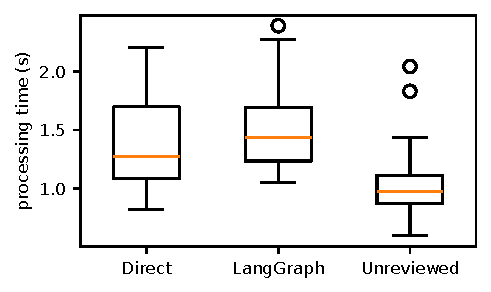
\includegraphics[width=\figscale{0.7}\linewidth]{figures/fig-orchestration.pdf}
\caption{Workflow processing time by execution mode on one machine with SQLite (O01).}
\label{fig:orchestration}
\end{figure}

Interruptions were injected at \V{O02-points} points in both modes with
\V{O02-trials} trials per cell (Table~\ref{tab:recovery}): transient failures and
simulated crashes (an exception bypassing the worker's handler followed by lease
expiry) during analysis, before recommendations, at a worker restart during review,
and during finalization. \textbf{In the evaluated interruption scenarios},
\V{O02-recovered} of \V{O02-runs} interrupted runs recovered to completion, and
\V{O02-identical} of them produced outputs identical to the uninterrupted
reference. Completed stages were repeated \V{O02-repeated} times; each run had
exactly one decision, one finalization and a verifying receipt. Real
process kills, network partitions and database failover were not exercised.

\widetable{tables/tab-recovery}

\section{External Validation and Failure Analysis}
\label{sec:external}

\paragraph{Setup.}
The unchanged pipeline analysed the UCI-498 incident log~\cite{amaral2018uci498},
a real IT service-desk event log of one organization, with each final assignment
group of sufficient size treated as an entity: \V{X02b-groups} groups,
\V{X02b-incidents} of \V{X02b-incidents-total} incidents, \V{X02b-events}
investigation-step proxies from work-state events and \V{X02b-reassign}
reassignment-based escalation proxies. The only available outcome is the final
service-level flag; SLA labels were loaded only after SAT-SA's ranking existed and
never entered a submission. \textbf{This is IT incident data, not SOC data.}
The same log has been used to model which factors predict meeting the SLA~\cite{swain2022sla};
we do not predict SLA attainment and use it only as an external outcome.

\paragraph{Feasibility.}
All \V{X02b-rows-received} submitted rows were accepted
(\V{X02b-rows-rejected} rejected) and every group's analysis completed, with a
median of \V{X02b-analysis-median}\,s per group on SQLite.

\paragraph{Negative result.}
SAT-SA's risk score was not associated with the SLA-miss rate: Spearman
$\rho=\V{X02b-rho-risk}$ (95\% bootstrap \V{X02b-rho-risk-lo} to
\V{X02b-rho-risk-hi}; Table~\ref{tab:external}, Figure~\ref{fig:external}).
Slowest median resolution reached $\rho=\V{X02b-rho-slowest}$
(\V{X02b-rho-slowest-lo} to \V{X02b-rho-slowest-hi}), which is expected because an
SLA miss is a timeliness outcome; reassignment rate reached
\V{X02b-rho-reassign} and volume \V{X02b-rho-volume}. Among the
\V{X02b-relevant} groups in the top SLA-miss quartile, SAT-SA's precision@10\% was
\V{X02b-p10-satsa} (random \V{X02b-p10-random}, slowest resolution
\V{X02b-p10-slowest}), and it needed to review \V{X02b-volume-satsa} groups to
find all of them (slowest resolution: \V{X02b-volume-slowest}).

% Generated by scripts/build_paper_assets.py from satsa-evidence-freeze-v2; do not edit.
% Sources: X02b=EXP-X02b-external-itsm (manifest 036652ed89089874)
\begin{table}[t]
\centering\small
\caption{External IT incident log (X02b): association with the SLA-miss rate over 50 groups of one organization.}
\label{tab:external}
\begin{adjustbox}{max width=\linewidth}
\begin{tabular}{lrr}
\toprule
Score & Spearman $\rho$ & 95\% bootstrap \\
\midrule
Incident volume & \ensuremath{-}0.15 & \ensuremath{-}0.42 to 0.16 \\
Reassignment rate & 0.37 & 0.08 to 0.60 \\
SAT-SA risk score & \ensuremath{-}0.11 & \ensuremath{-}0.42 to 0.21 \\
Slowest median resolution & 0.94 & 0.86 to 0.97 \\
\bottomrule
\end{tabular}
\end{adjustbox}
\par\smallskip\footnotesize Top-quartile precision@10\%: SAT-SA 0.40, random 0.25, slowest resolution 1.00. Not SOC data.
\end{table}


\begin{figure}[t]
\centering
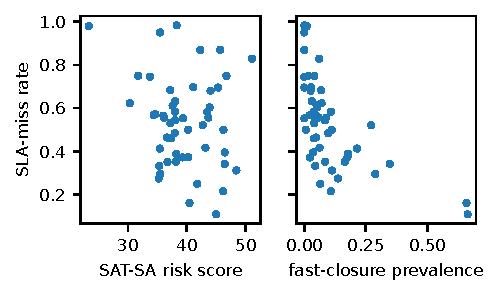
\includegraphics[width=\linewidth]{figures/fig-external.pdf}
\caption{External IT incident log: SAT-SA risk versus SLA-miss rate (left) and
fast-closure prevalence versus SLA-miss rate (right), one point per group
(X02b, X03). Not SOC data.}
\label{fig:external}
\end{figure}

\paragraph{Failure analysis.}
A diagnostic analysis (X03) on the same data changed no detector, threshold or
weight. It attributes the result to four causes.
\emph{(1) Construct mismatch (primary).} The prevalence of fast closures was
negatively associated with SLA misses ($\rho=\V{X03-rho-fast}$,
\V{X03-rho-fast-lo} to \V{X03-rho-fast-hi}): on a service desk fast resolution is
the goal, whereas SAT-SA treats fast closure of security alerts as possible skipped
investigation. The execution-gap dimension, which this signal drives, correlated at
$\V{X03-rho-execgap}$ (\V{X03-rho-execgap-lo} to \V{X03-rho-execgap-hi}).
\emph{(2) Existence-rule saturation.} In total, \V{X03-saturated} detector
families fired for every group, although their input conditions varied widely---cases without any
step \V{X03-cases-min} to \V{X03-cases-max} of cases, medium-or-higher alerts with
fewer than two steps \V{X03-alerts-min} to \V{X03-alerts-max}. A rule that fires on
``at least one'' qualifying record cannot discriminate submissions with thousands
of tickets, and the fusion adds near-constant amounts for these families because it
ignores prevalence. Risk still took \V{X03-risk-distinct} distinct values and was
unrelated to volume ($\rho=\V{X03-risk-vs-volume}$).
\emph{(3) Unavailable constructs.} Of the \V{CODE-dimensions} risk dimensions,
\V{X03-zero-dims} had no input data; investigation steps and escalations are proxies (state changes and
reassignments), and monitoring coverage is unavailable.
\emph{(4) An adapter artifact.} The log has no step notes; the adapter submits
empty notes, which satisfy the repeated-investigation note rule in
\V{X03-note-rule} groups.

The analysis found no temporal or label defect: risk and label cover the same
incidents and period; only \V{X03-other-group} of \V{X03-missed} SLA misses
occurred while another group held the ticket; and reassigned incidents missed
more often (\V{X03-reassigned-miss} versus \V{X03-notreassigned-miss}),
consistent with the positive reassignment association. The one pipeline defect
found---ingestion totals recorded as null---affected bookkeeping only; its fix
produced X02b with identical analytical outputs.

\paragraph{Decision and interpretation.}
No risk-model change was made. A change that raised the correlation with SLA
misses would optimize SAT-SA toward a timeliness construct it does not claim to
measure, using the evaluation data for tuning. We therefore read X02b and X03 as
\emph{feasibility and construct-validity evidence rather than external-effectiveness
validation}: the unchanged pipeline processed real workflow data, and on data
whose outcome measures a different construct and lacks investigation, escalation
and coverage semantics, SAT-SA's supervisory signals did not transfer. The
prevalence-blind fusion of existence rules is a design limitation in SAT-SA's own
domain; addressing it needs SOC development data held out from evaluation.

\section{Security and Integrity Evaluation}
\label{sec:integrity}

\paragraph{Threat model.}
TRUST-SAT targets after-the-fact alteration of the supervisory record: someone
with write access to the database or ledger file changes a decision, finding,
risk profile, recommendation, source record or receipt after the supervisor
decided. It does not address compromise of the signing key, of the running
process before finalization, of the operating system, or submission of false
records by the monitored organization; it binds what was analysed and decided,
not whether the submitted records are true.

\paragraph{Mechanism.}
Finalization serializes a canonical document of the reviewed state (decision,
findings, observations, risk, recommendations, submission records and their
provenance), hashes it with SHA3-256~\cite{nist2015fips202}, signs the digest with
\V{CODE-signature}~\cite{nist2024fips204}, and appends a ledger entry whose hash
covers its predecessor, in the spirit of tamper-evident logging~\cite{schneier1999logs,crosby2009logging}.
Verification rebuilds the document from the live database, compares digests,
checks the decision binding, the signature against the stored public key and the
ledger chain.

\paragraph{Mutation matrix (RQ5).}
On one finalized controlled workflow, each of \V{T01-tested} mutations was applied,
verified, restored and re-verified (Table~\ref{tab:trust}). Verification detected
\V{T01-detected}/\V{T01-expected} tested mutations of signed state---decision action
and reason, finding, risk, recommendation, observation scope, source provenance,
submission record payload, artifact digest, canonical payload, receipt signature,
receipt public key and ledger chain. The negative control (\V{T01-controls} case), a
mutation of an unsigned operational queue field, still verified, as designed. This is evidence
that the tested mutations are detected, not a detection rate and not prevention: an
attacker able to rewrite the database and re-sign with the service key, or to
substitute a key pair consistently across receipts and ledger, is outside the model
unless the public key is pinned out of band. Key management and
rotation were not evaluated.

\widetable{tables/tab-trust}

\paragraph{Tenant isolation and access.}
Submission, analysis, review and verification are scoped by tenant; the peer
worker uses only same-tenant cohorts; only the supervisor or administrator role can record a
decision. These properties are covered by the automated test suite rather than by
a dedicated experiment and were not subject to adversarial testing.

\section{Discussion}
\label{sec:discussion}

\paragraph{What the evidence supports.}
Under controlled conditions the mechanisms behave as designed: declared finding
families are emitted with evidence references, the ranking separates generated
pathological entities from random and volume orderings, validation follows its
declared contract, the tested integrity mutations are detected, and the evaluated
interruptions recover without duplicated decisions. These are mechanism-level
claims. On independent real data the pipeline is feasible end to end.

\paragraph{What it does not support.}
It does not show that SAT-SA improves supervision. Simple rules tie the fast-closure
detector and nearly match the prioritization; the controlled data and labels are
SAT-SA's own; the only independent outcome available was a different construct,
and there SAT-SA's risk showed no association. No supervisor used the system in a
study, and no expert labelled findings. The honest reading is that SAT-SA is a
working, inspectable pipeline whose \emph{usefulness} is untested.

\paragraph{Why the simple baselines matter.}
The closure-speed heuristic tied or nearly tied SAT-SA in most populations,
which is consistent with a generator whose pathological profile includes fast
closures (we did not isolate the cause). More elaborate
workers can only earn their place against data where pathologies are not
separable by one rate; the ablation's finding that four workers \emph{lowered}
population recall points the same way. For a supervisor, a small set of transparent
rates may be a reasonable first instrument, with record-level findings as the
explanation layer rather than the ranking signal.

\paragraph{Design lessons from the negative results.}
Three design properties surfaced. (i) Existence rules plus confidence-only fusion
saturate on large submissions; prevalence-aware scoring is a candidate
intervention, to be developed on held-out SOC data rather than on UCI-498.
(ii) All-or-nothing validation protects analysis from inconsistent data but turns
modest record loss into rejection of a whole period. (iii) No period, recency or
consistency checks exist, so stale and contradictory records pass silently---a gap
for any supervisory use where submissions are adversarial.

\paragraph{Role of orchestration and of the human.}
The analytics are deterministic; LangGraph provides checkpointed sequencing and a
review interrupt, at a small cost on this workload, and does not make analytical
decisions. SAT-SA is decision support: the supervisor decides, and TRUST-SAT records
what was decided on which evidence. Automation bias~\cite{parasuraman2010automation}
is a real risk for such tools and was not studied.

\paragraph{Contribution strength.}
The empirical findings, including the negative ones, and the reproducibility
infrastructure are the most defensible contributions. The integrity layer is an
integration of standard primitives. The application framing is a low-confidence
candidate: our literature search was structured but not systematic, and it found
close prior work on automated, record-based assessment of incident handling for
auditors~\cite{palma2024compliance}.

\section{Limitations and Threats to Validity}
\label{sec:limitations}

\paragraph{Construct validity.}
Controlled labels are construction labels written by the system's authors; they
encode what scenarios were built to contain. The external outcome (SLA miss)
measures timeliness, not supervisory execution quality, and investigation and
escalation are proxies there. Risk scores have no validated meaning as
probabilities or severities.

\paragraph{Internal validity.}
Populations for prioritization and ablation come from SAT-SA's own generator,
which injects the behaviours its detectors target, favouring SAT-SA. Precision
depends on database layout (shared versus isolated). Detector thresholds were set
by design, not fitted; we made no changes on evaluation data, but they were also
never tuned on independent development data.

\paragraph{External validity.}
There is no SOC data from a real organization. The external dataset is one IT
service desk. Generated populations have \V{PR01-entities} entities, making top-$k$
estimates coarse. The ablation population analysis uses five seeds and is
exploratory.

\paragraph{Statistical conclusion validity.}
Intervals are descriptive, seeded and uncorrected across many comparisons; no
hypothesis test is made. Orchestration measurements are repeated runs on one
machine and do not generalize across hardware, databases or load. Recovery was
tested with injected exceptions at worker-method boundaries, not real process
kills, partitions or database failover.

\paragraph{Human factors.}
The human evaluation protocol is ready but \textbf{the study was not executed};
there are no participants and no usability or decision-quality results. The expert
label pipeline is ready, but \textbf{no expert-labelled data exist}.

\paragraph{Security.}
Integrity results cover \V{T01-expected} tested mutations on one workflow; key
compromise, key management, insider re-signing and false submissions are out of
scope. Tenant isolation was not tested adversarially.

\paragraph{Deployment.}
All measurements used SQLite and local storage on one machine. The local API and
worker processes passed \V{D01-pass} HTTP smoke checks (\V{D01-fail} failed,
\V{D01-notrun} not run). Docker was not installed, so container images and the
compose topology were not executed; PostgreSQL was not live-tested (no connection
string was available); SeaweedFS object storage and the CI topology job were not
executed; no hosted deployment exists (Table~\ref{tab:deployment}). No claim of
production readiness or scale is made.

\widetable{tables/tab-deployment}

\section{Reproducibility}
\label{sec:repro}

\paragraph{Evidence chain.}
Each reported number is a \verb|\V{claim-id}| macro generated by the paper data
layer from a canonical bundle in the evidence freeze
\texttt{satsa-evidence-freeze-v2}; the build verifies each bundle's hashes against
the freeze before reading it. Tables and figures are generated the same way and
record their source bundles and manifest hashes. An audit script regenerates paper
data, tables and figures and compares them byte for byte with the committed files,
rejects undefined macros and hand-typed decimals, checks that every citation is a
verified row of the literature matrix, and scans for prohibited claim wording.
The package is archived as a write-once publication snapshot that records the
hash of the freeze it was generated from and the hash of every file.

\paragraph{Reproduction levels.}
We classify what has actually been demonstrated:
\begin{itemize}
\item \emph{Level 1, artifact verification (demonstrated):} the freeze verifier
  recomputes every recorded hash; it has passed in the working repository and in a
  fresh clone, and a mutation drill showed that edited manifests, raw results,
  metrics and configurations are rejected.
\item \emph{Level 2, result regeneration (demonstrated):} paper tables, figures and
  values regenerate byte-identically from the frozen bundles, and the freeze's
  exports regenerate identically.
\item \emph{Level 3, experiment reproduction (demonstrated for deterministic
  experiments):} re-running the integrity mutation matrix (T01) and the peer sweep
  (P01) from the recorded code under new experiment identifiers reproduced their
  analytical outputs; timing-based experiments reproduce only in distribution.
\item \emph{Level 4, environment reproduction (not demonstrated):} a container
  image and compose topology exist but were not executed; all runs used one
  Windows machine with the project's Python dependencies.
\item \emph{Level 5, external-data reproduction (demonstrated once):} the external
  experiment was executed twice from the public dataset (X02, since superseded, and X02b, at different
  commits) with identical analytical outputs; it has not been reproduced by a third
  party.
\end{itemize}

\paragraph{Commands.}
All commands are Python scripts in the repository's \texttt{scripts} directory.
Level~1 runs \texttt{verify\_\allowbreak evidence\_\allowbreak freeze.py} on the
freeze; Level~2 runs \texttt{build\_\allowbreak paper\_\allowbreak assets.py} and then
\texttt{audit\_\allowbreak paper.py}; Level~3 re-runs
the experiment runners with each bundle's recorded configuration. The supplementary
material lists the full commands, seeds, dataset provenance and what cannot be
reproduced.

\paragraph{Code, data and artifact availability.}
The SAT-SA source code, experiment runners, evidence freeze, paper data layer and
the literature-search scripts are in the project repository under the MIT licence
(\url{https://github.com/PrathamKapoor/SAT-SA-with-PQC}); the commit that
contains this manuscript and the publication snapshot is identified in the
supplementary material. All controlled data are synthetic and regenerate from the
recorded seeds and configurations. The external dataset~\cite{amaral2018uci498}
is public under a Creative Commons Attribution (CC BY) licence and is not
redistributed; the experiment downloads it
and verifies its checksum. No personal data, no data from a real SOC and no
human-participant data were used.

\section{Conclusion}
\label{sec:conclusion}

SAT-SA turns the operational records a monitored SOC submits into evidence-cited
supervisory findings and priorities, keeps the decision with a human supervisor and
binds that decision to the analysed state. A frozen, hash-verified evaluation shows
the mechanisms working under controlled conditions and the pipeline running on real
external data. It also shows where they fall short: simple rules match much of the
controlled performance, stale and contradictory evidence passes silently, and on an
IT incident log the supervisory risk did not track the only outcome available,
mainly because that outcome measures a different construct. The next evidence
needed is not more controlled experiments but SOC records with independent outcomes,
expert-labelled findings and a study with supervisors.


\section*{Acknowledgment}
% IEEE policy (verified 2026-09-27): "The use of content generated by artificial
% intelligence (AI) in an article (including but not limited to text, figures,
% images, and code) shall be disclosed in the acknowledgments section"; the AI
% system and the sections, with the level of use, must be identified.
% AUTHORS: confirm or correct this statement before submission (see
% paper/VENUE_COMPLIANCE.md, row "AI disclosure"). It states the preparation
% history recorded for this manuscript; do not remove it without replacing it
% with an accurate statement.
The authors used an AI system, Claude (Anthropic), through the Claude Code tool, in
preparing this article. It drafted the text of all sections. It wrote the code that
runs the experiments, generates every table, figure and reported value from the
frozen evidence, and performs the literature searches. It also screened the search
results for Section~\ref{sec:related}. Reported numbers are not typed by hand; they
are generated by that code from hash-verified experiment bundles.
[AUTHORS: state here how you reviewed and edited the AI-generated content and that
you take responsibility for it.]

\bibliographystyle{IEEEtran}
\bibliography{references}

\begin{IEEEbiographynophoto}{PrathamKapoor}
[Biography to be supplied by the author: degrees, current position, research
interests, as required by IEEE Access for all authors.]
\end{IEEEbiographynophoto}

\EOD

\end{document}
